\documentclass[12pt]{article}
\usepackage{cite}
\usepackage{color}
\usepackage{graphicx}
\usepackage{caption}
\usepackage{subcaption}
\usepackage{parskip}

\setlength{\parskip}{5pt}
\setlength{\parindent}{0pt}

\title{LC/MS Chromatogram Smoothing With Generative Adversarial Networks}

\author{Gabriel Ferns(CS Senior) , Max Horowitz-Gelb(CS Senior)}

\begin{document}

\maketitle

\abstract{
Liquid Chromatography Mass Spectrometry is a powerful tool for identifying and quantifying proteins in a complex sample. High throughput methods for LC/MS allow allow for analysis of samples with thousands of proteins. But this increase in throughput comes at the cost of a decrease in signal quality. This issue calls  for post extraction methods to clean and smooth chromatogram signal data. Here , using a new and powerful deep learning framework known as GANs \cite{GAN}, we attempt to smooth chromatograms, without distortion of the true underlying quantifiable data. 
From our experiments we show promising results which are able to somewhat achieve the same shape as our input while not distorting the quantifiable data.

\section{Introduction}
DIA \cite{DIA} is a method of LC/MS for quanitifying thousands of proteins in a single sample. In order to analyze thousands of proteins at the same time, DIA requires a low sample rate. This results in the quality of the data extracted to be quite poor. An alternative to DIA is SRM, or Selected Reaction Monitoring,\cite{SRM}. SRM is not good for quantifying more than a handful of peptides at a time, but the data generated is of far superior quality. It would be nice if we could keep the high throughput of DIA while also having data with the same quality as SRM. Then one could analyze thousands of proteins at the same time and get clean reliable data for quantification.

The quality of SRM data in comparison to DIA data suggests that perhaps a generative model trained on clean SRM data, could remove noise and smooth DIA data without distorting the actual quantifiable information. To test this hypothesis we chose to use a GAN as our generative model. GAN neural networks have been shown as powerful tools for image processing particularly for removal of noise and upscaling of images \cite{SRGAN}\cite{DE_RAIN}. We applied similar methods to chromatogram data by training a GAN on clean SRM dataset with simulated Gaussian noise. We then tested our GAN on a dataset of real DIA data. Unfortunately our GAN model was not able to smooth the input. But it was able to somewhat learn a compression of the input space and output chromatograms with similar shape to the input without distorting quantifiable data.



\begin{figure}
\centering
\begin{subfigure}{.5\textwidth}
  \centering
  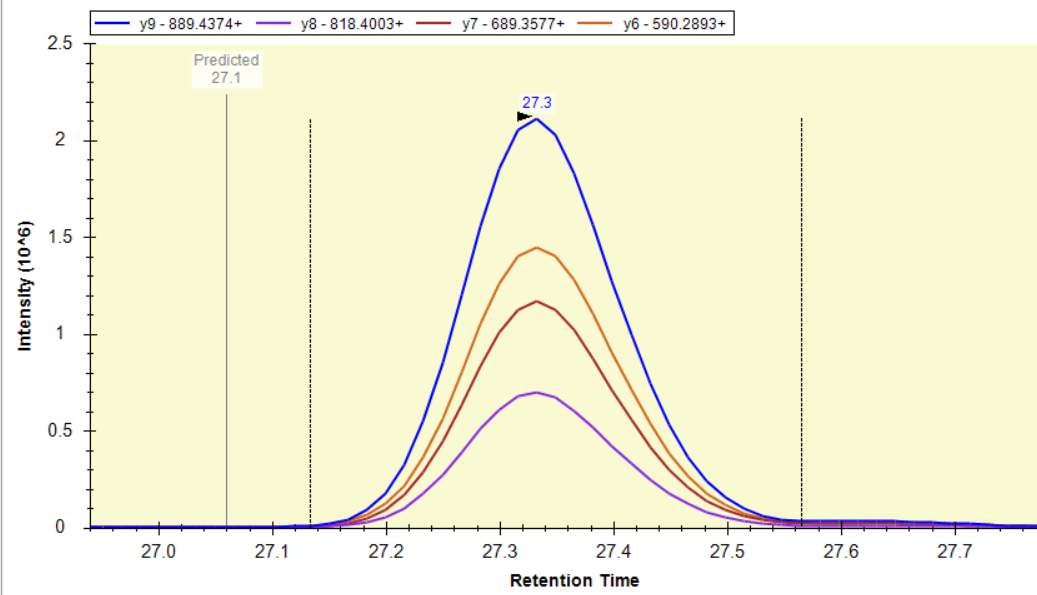
\includegraphics[width=1\linewidth]{smoothExample.png}
  \caption{SRM Chromatogram}
  \label{fig:sub1}
\end{subfigure}%
\begin{subfigure}{.5\textwidth}
  \centering
  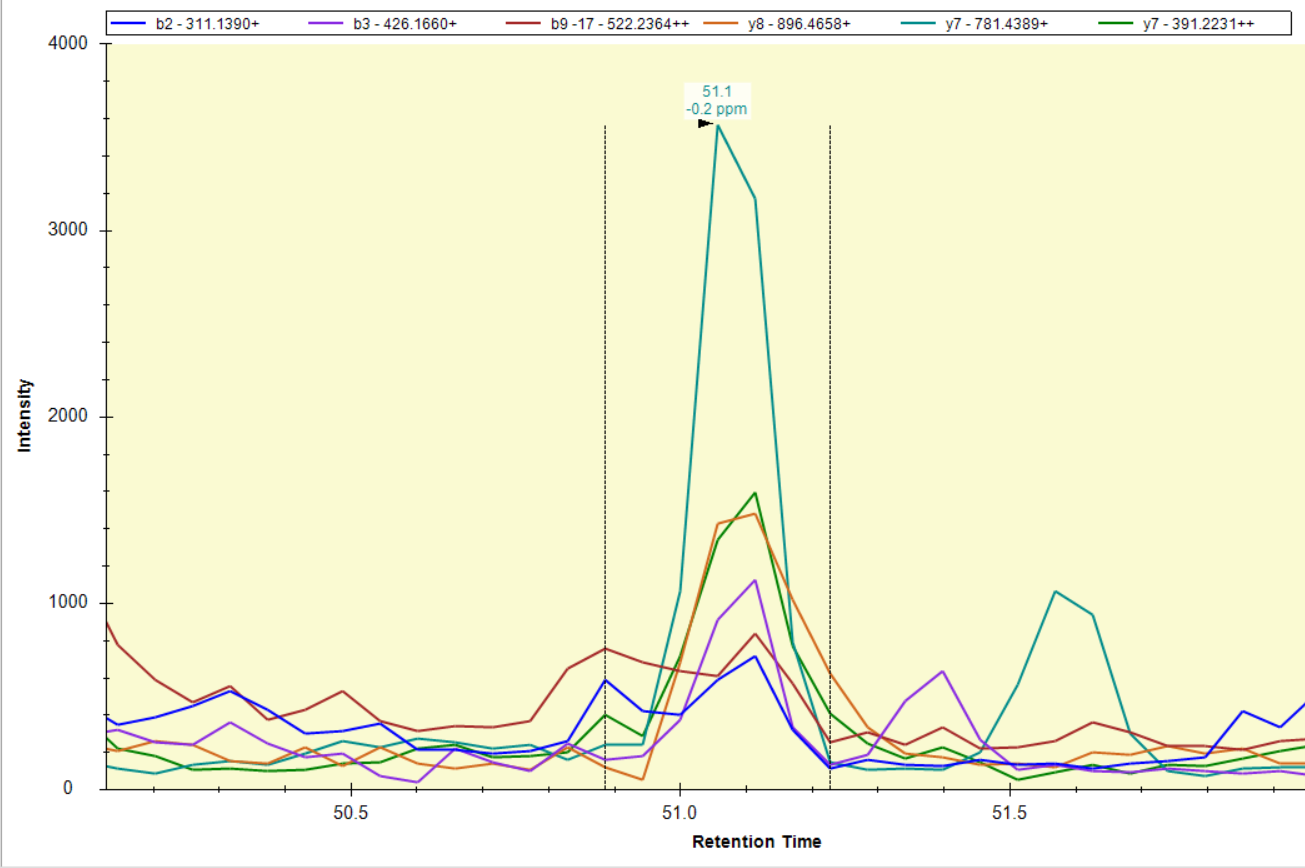
\includegraphics[width=1\linewidth]{DIA_example}
  \caption{DIA Chromatogram}
  \label{fig:sub2}
\end{subfigure}
\caption{Here we show two chromatograms. As one can see the noise and the smoothness is much better in the chromatogram coming from an SRM dataset.}
\label{fig:test}
\end{figure}

\section{Brief LC/MS Primer}
LC/MS identifies and quantifies proteins by separating them by their hydrophobicity and mass. In general it is difficult to quantify whole proteins so we instead use peptides, which are sub-sequences of a protein. These peptides come off of a liquid column at a specific time which is dependent on the hydrophobicity of the peptide. This time is known as the peptide's Retention Time. Once the peptide comes off the column it is ionized and then becomes what is called a precursor ion. When precursor ions go into the mass spectrometer they are filtered by the ratio of their mass to charge. A precursor ion's mass to charge along with its retention time are used as a two fold filtration process for unique identification and quantification of peptides. 

At this point one could start quantifying the peptide, but in certain methods, like DIA, the precursor is then blasted it with an ion spray. This ion spray causes the precursor to fragment into two pieces. One of these pieces, known as a transition ion, becomes charged and may be detected by the machine. The fraction of the time the machine detects any possible fragment is relatively stable and known from empirical data. Because of this the relative ion intensity of each transition ion is useful for identification of the peptide. The relative intensity of each ion can be thought of as a unique key for a peptide.

\begin{figure}
\centering
\begin{subfigure}{.5\textwidth}
  \centering
  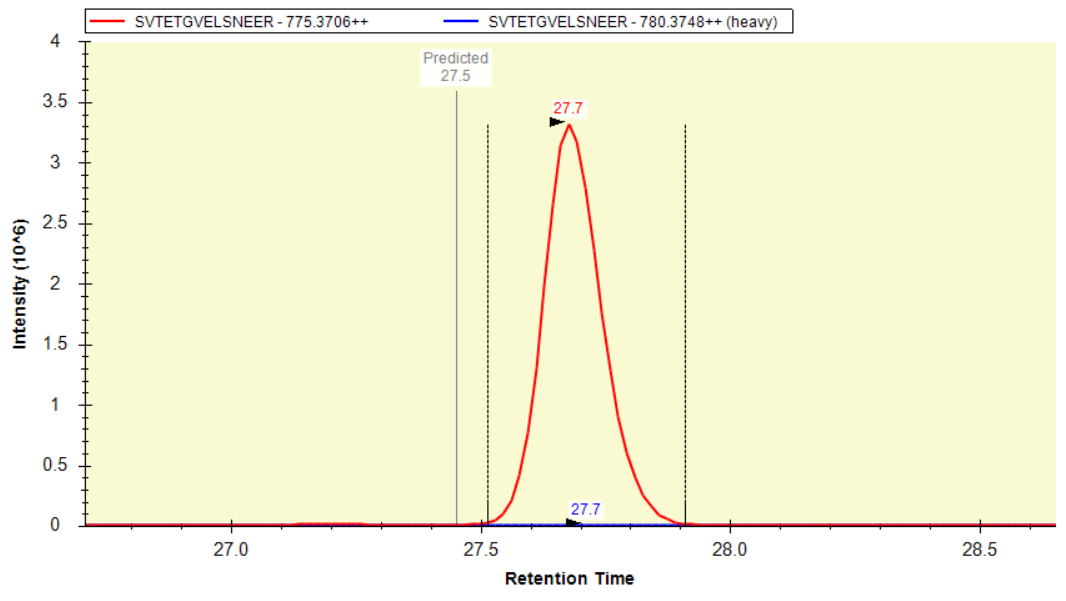
\includegraphics[width=1\linewidth]{precursor}
  \caption{Precursor Chromatogram}
  \label{fig:sub1}
\end{subfigure}%
\begin{subfigure}{.5\textwidth}
  \centering
  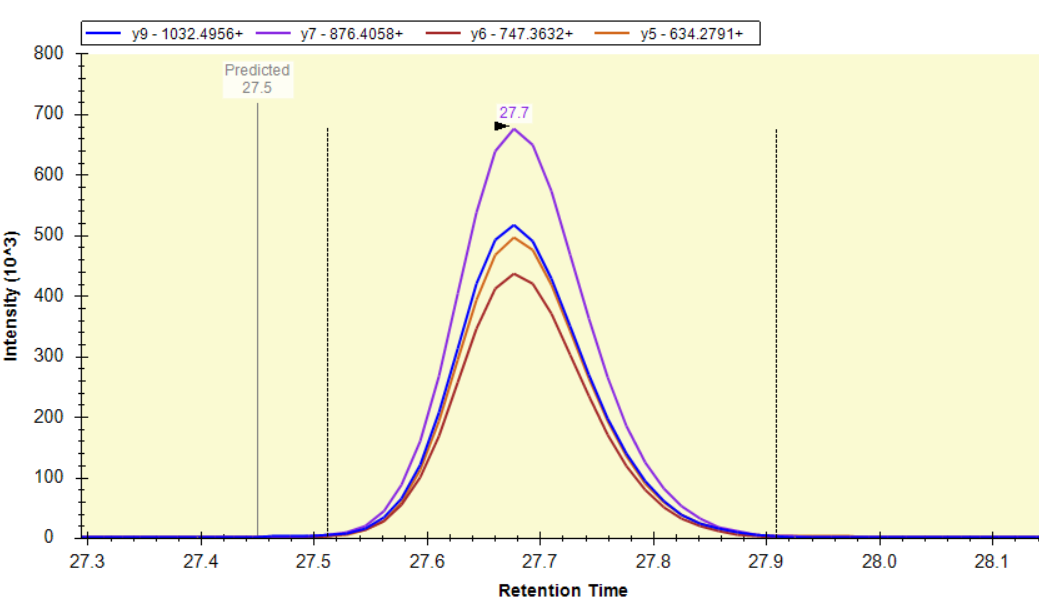
\includegraphics[width=1\linewidth]{transitions}
  \caption{Transition Chromatograms(Peak Group)}
  \label{fig:sub2}
\end{subfigure}
\caption{Here we show the difference between precursor and transition ion chromatograms. The precursor chromatogram contains a single peak, while the transition chromatogram shows a set of peaks coming from all the different transitions or fragment ions. This set of transition chromatograms coming from the same peptide is known as a peak group.}
\label{fig:test}
\end{figure}


\section{Task Definition}
The goal of this project is to train a GAN so that it can take a peak group and return the same peak group after being smoothed and denoised.  
The GAN smooths and denoises each transition separately. The network takes as input the chromatogram from a single transition as well as an average signal from all the other transitions coming from the same peak group.  The reason this is done is that, as one can see from figure 2b, each transition chromatogram has a similar shape to all the other chromatograms in the same peak group. So having an average of the other chromatograms is a clue into the true shape of the transition chromatogram we are trying to smooth. 

The GAN takes the average chromatogram and the single transition chromatogram as input and then outputs a chromatogram of the single transition after it has been smoothed. 

\begin{figure}
\centering
\begin{subfigure}{.5\textwidth}
  \centering
  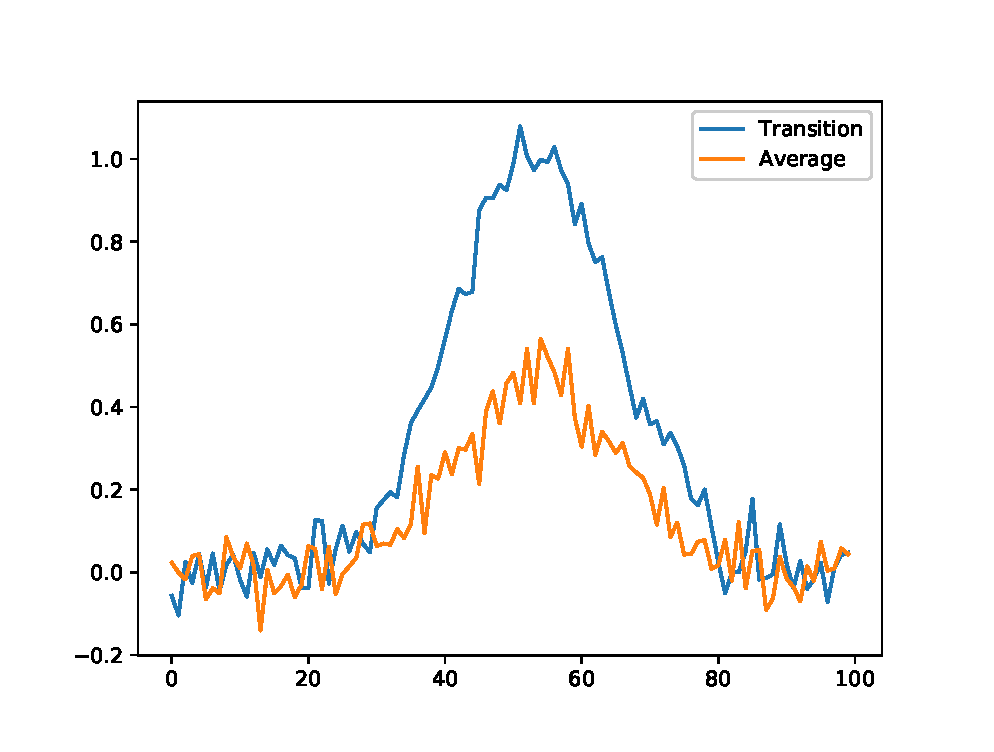
\includegraphics[width=1\linewidth]{input}
  \caption{Input}
  \label{fig:sub1}
\end{subfigure}%
\begin{subfigure}{.5\textwidth}
  \centering
  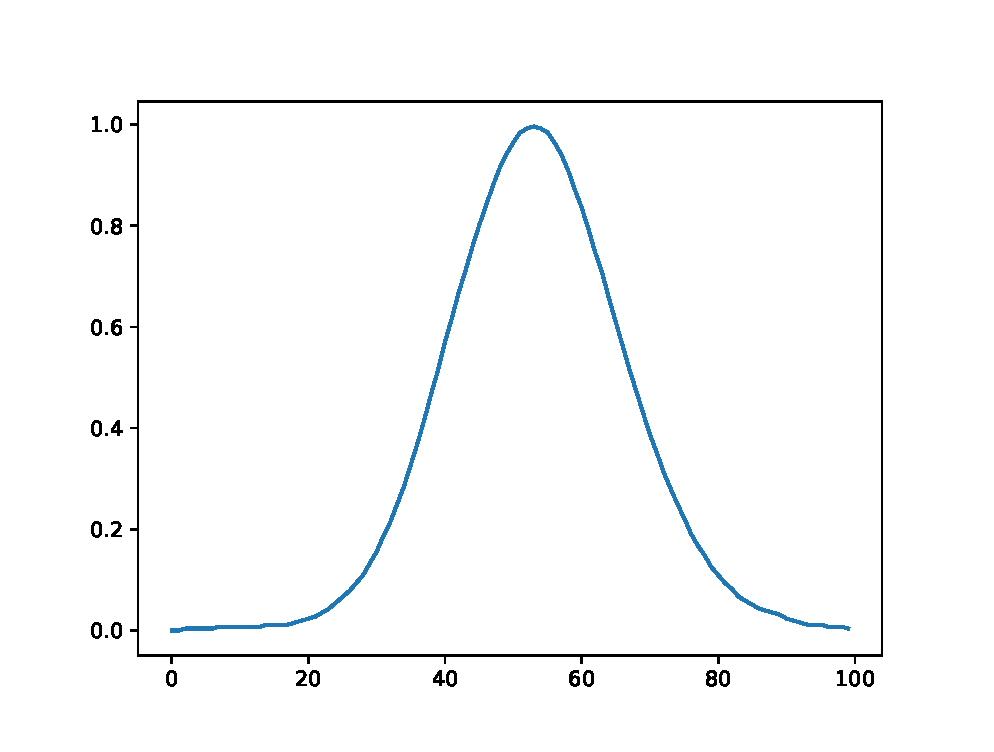
\includegraphics[width=1\linewidth]{output}
  \caption{Output}
  \label{fig:sub2}
\end{subfigure}
\caption{Here we show the input and output data for the GAN network. The input composes of unique transition along with an average shape chromatogram coming from all other transitions in the peak group. The output is the smoothed peak group from the transition. (Note the above is not real input or output data as a result of training. It is only for demonstration)}
\label{fig:test}
\end{figure}


\color{black}

\section{Algorithm Definition}
\subsection{Chromatogram Pre-processing}
Before we can use the chromatogram data it has to be pre-processed. The time span of each peakgroup was not of equal length so all the chromatograms had to be up-sampled or down-sampled so that they were all a standard length of 100 intensity points per peak. As well the intensities were normalized to range from 0 to 1.   
\subsection{GAN}
With this processed data, we trained a 1-Dimensional, denoising GAN. Because the
data is effectively a 1-Dimension Image, we chose to adapt a popular
Convolutional GAN architecture that has been successfully applied to images, known as DCGAN.

\subsection{Noise Model}
In order to remove the effect of the noise on the activation, we need to be able to
generate examples of this noise. The best noise model would be the actual,
underlying physical process. We do not have access to this, however, so we
defined a noise model that is a Gaussian Process with an RBF Kernel with
dimension 1. The advantage of our approach over just assuming some generative
model for the peptide activation is that a noise model will potentially be
much simpler because it depends on the data collection apparatus and not the
structure of the peptide.

\subsection{Architecture Decisions}
In general, we used the architecture advice present in \cite{GAN}, with several
alterations to fit our specific problem domain. Neither the discriminator, nor
the generator has any type of pooling layer because the operation we want is
smoothing, and there should be no ``nonlocal-information'' that would
necessitate summary statistics from a pooling layer. Also, pooling layers have
been shown to hurt convergence \cite{GAN}. Batch normalization was used in both
the Generator and the Discriminator, as were LeakyReLUs.

\subsection{Generator Architecture}
\begin{center}
\begin{figure}
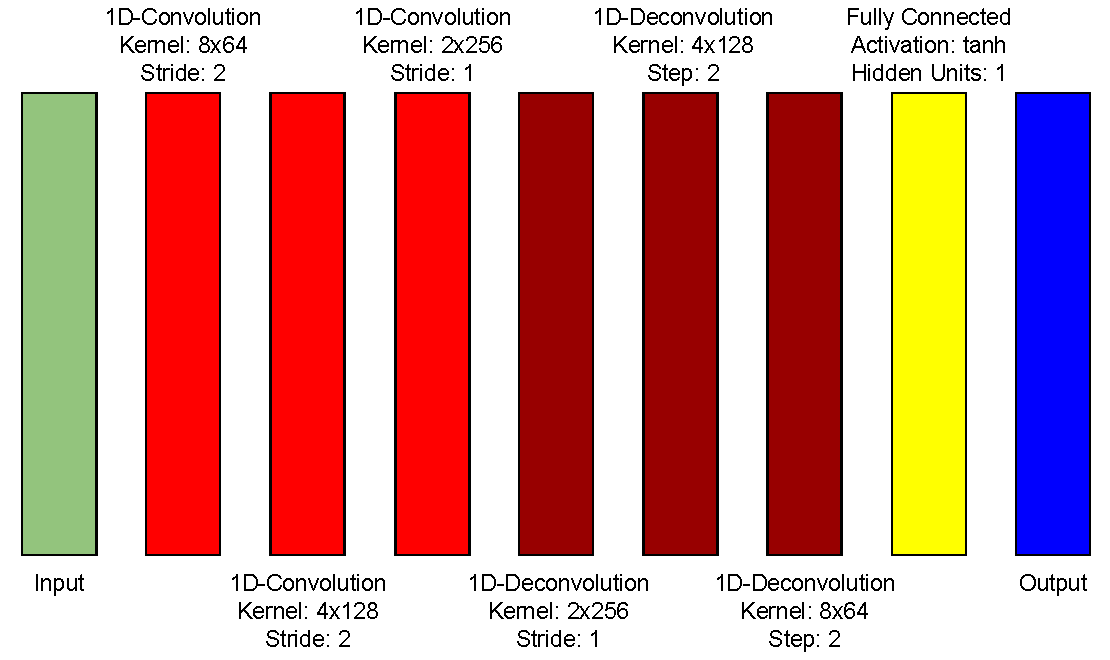
\includegraphics[scale=0.5]{TopoGenerator}
\caption{Generator Structure}
\end{figure}
\end{center}
The Noise Model is sampled and added to a real example, and then fed into the
generator. The Generator will then attempt to reconstruct the original image,
minus the noise. The loss function on the generator is the squared difference
between the denoised output image and the original image, and the standard
$log(D)$, where $D$ is the Discriminator's loss.
Gradient Descent was achieved using the ADAM optimizer with $\epsilon=0.01$. The
number of parameters in the Generator decreases near the center of the network,
in order to force it to generalize. We used dropout with $p=0.5$ in both the
training and testing of the Generator.

\subsection{Discriminator Architecture}
\begin{center}
\begin{figure}
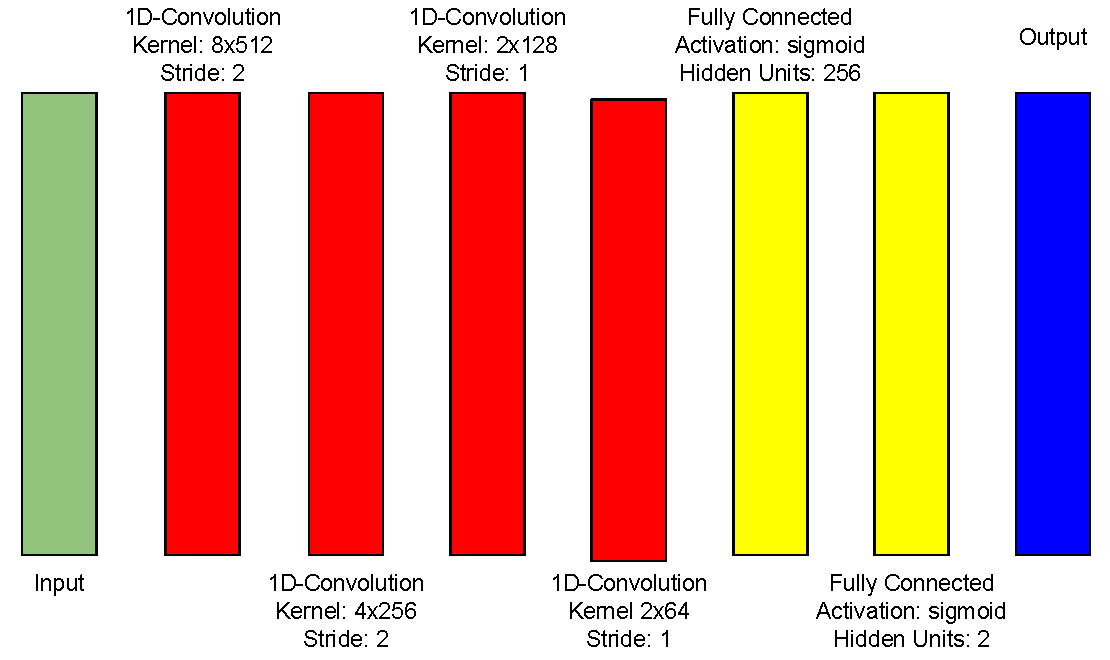
\includegraphics[scale=0.5]{TopoDiscriminator}
\caption{Discriminator Structure}
\end{figure}
\end{center}
The inputs to the Discriminator are either images that come from the
generator, or the real noiseless images, and it is the job of the Discriminator
to distinguish between the two. Stochastic Gradient Descent with a learning rate
of $\eta = 0.01$ was used to optimize the weights of the network.


\section{Methodology}
For training we used a high qualitiy SRM dataset\cite{Smooth_data} containing approximately 12,000 unique transition chromatograms. For our testing, we used DIA dataset \cite{TRIC} of 16 samples each containing 500 peakgroups.

For the test data, we only had the noisy raw DIA data. We don't know what the true shape of the peaks should look like once the noise was removed. For a single peak group the only way to know if we correctly smoothed the data without distorting it would be if we knew beforehand the true amount of protein that existed in the sample. Unfortunately we did not know that for the samples we were using so we had to use a different metric. 

Instead we used relative ion intensity to measure the quality of our data. As mentioned earlier in the primer, the relative intensity of each fragment ion has a fairly stable value which we can use for identification. In the test set we have 16 different samples all containing the same peptides. If after smoothing the test data we found that the relative ion intensties for the same peptide across samples didn't match, then we would know that we had corrupted the data. 

To calculate this metric we simply integrate over the curve of each ion's chromatogram in the same peak group. Combing these integrations gives a vector of chromatogram areas for each peptide in each sample. Then with these vectors we simply calculate the average cosine angle between all different samples for the same peptide. This average is our score, where 1 is the best and -1 is the worst.

If after doing smoothing from GANS we see this score go significantly down from before smoothing, then we know that we are corrupting the data. But if it is close to 1, then we can feel confident that the GAN is smoothing the data correctly. 
\section{Results}

In the test set we achieved images that appeared to somewhat look like the original input. The data was also not corrupted. Both the original DIA data and the predicted data got approximately the same dot product scores of $\sim 0.98$. 

\section{Test Predictions}
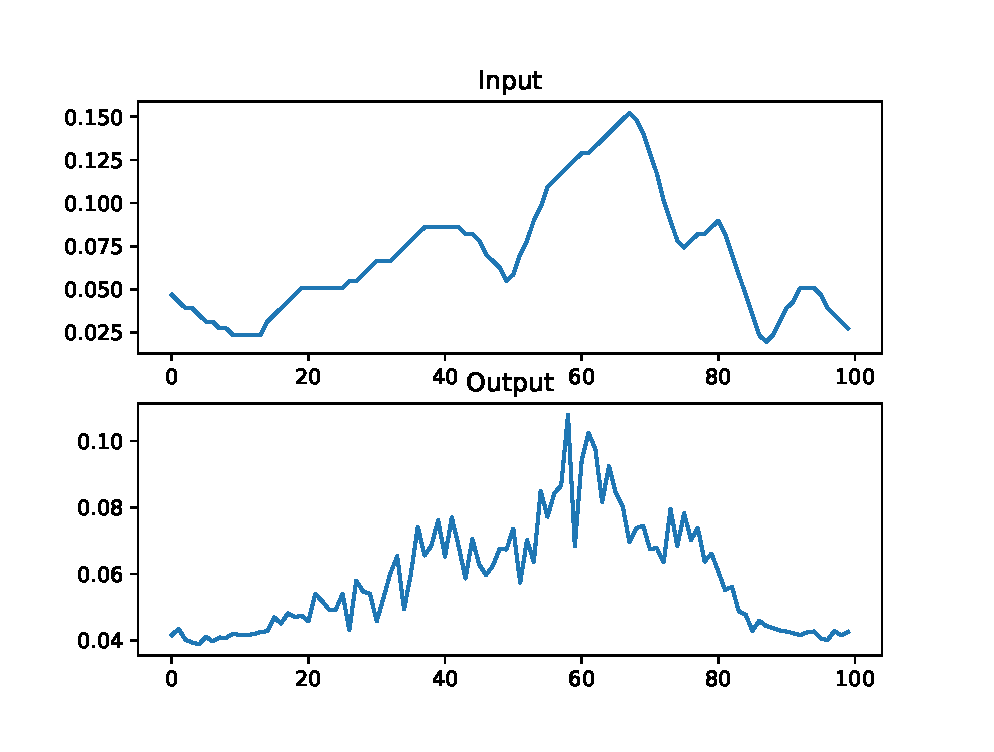
\includegraphics[scale=0.5]{example1}
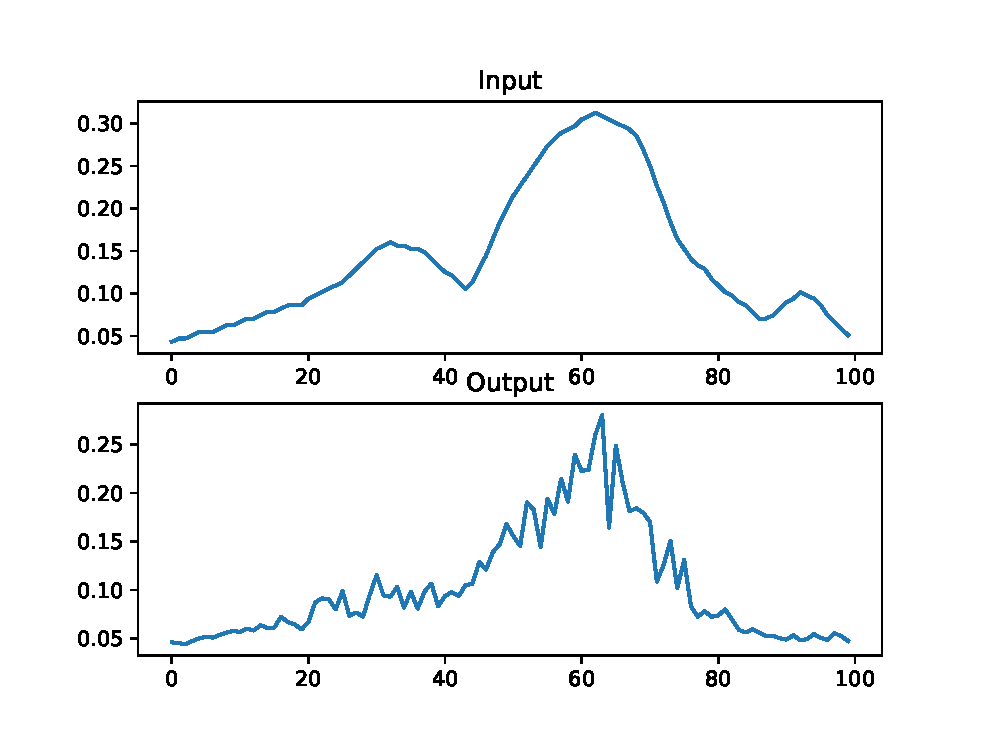
\includegraphics[scale=0.5]{example2}
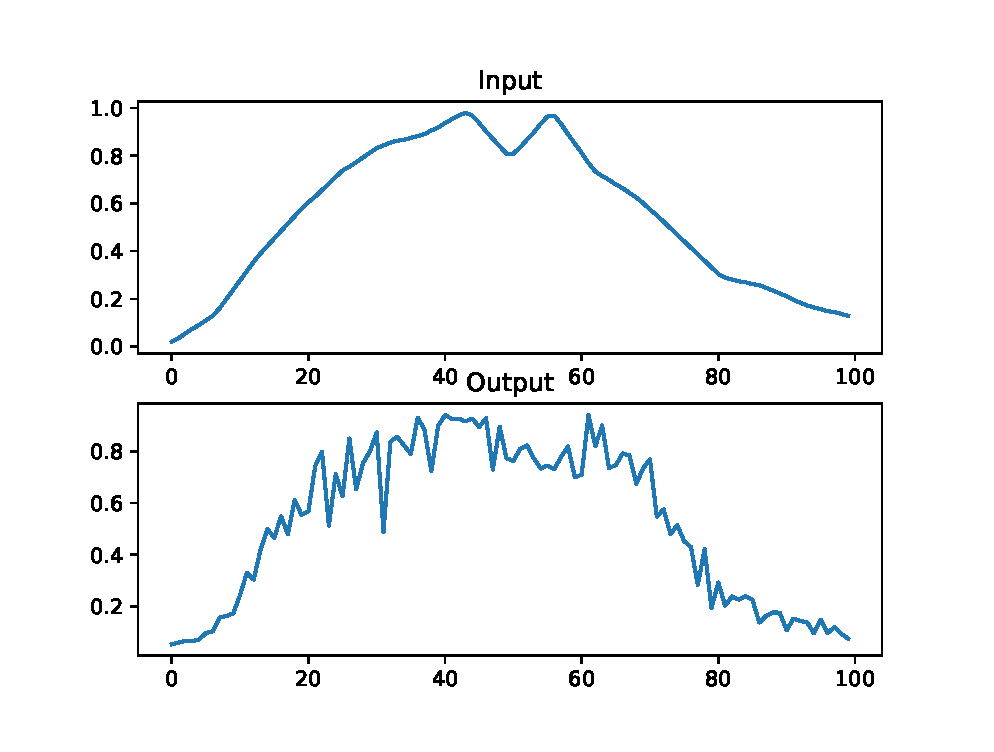
\includegraphics[scale=0.5]{example3}
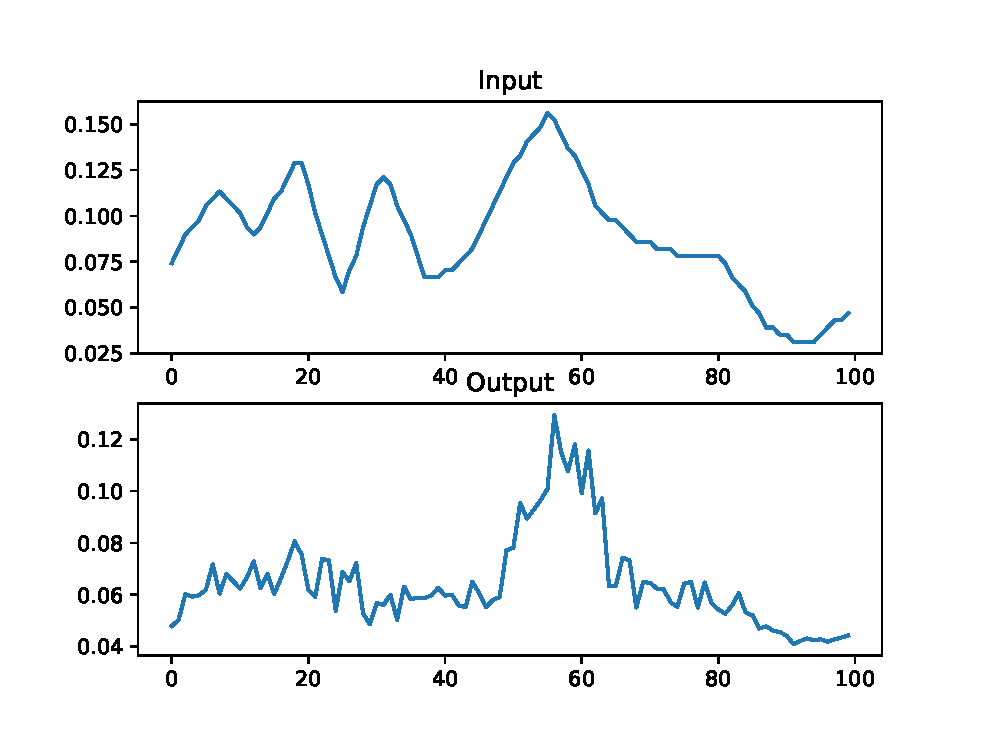
\includegraphics[scale=0.5]{example4}
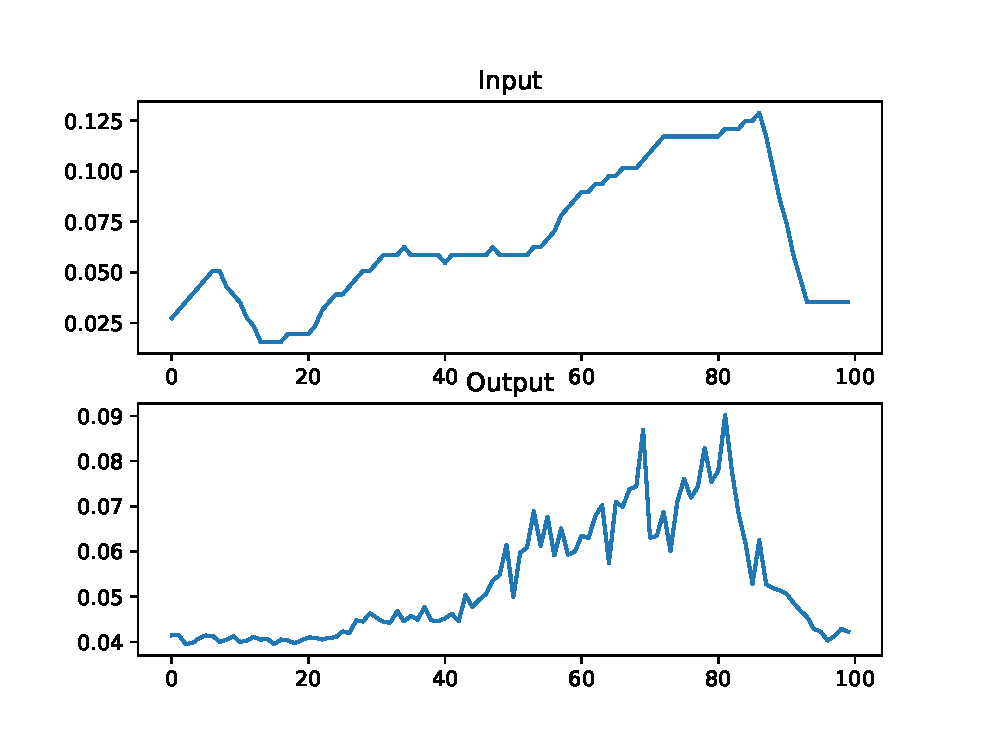
\includegraphics[scale=0.5]{example5}
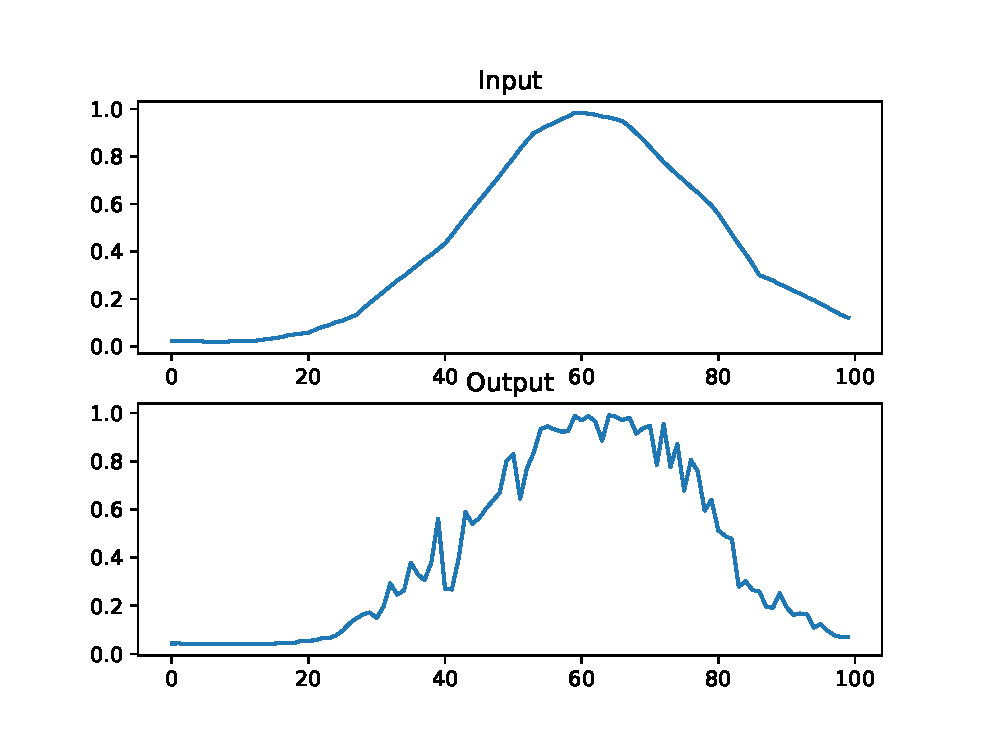
\includegraphics[scale=0.5]{example6}

\section{Discussion}
In previous efforts, groups have used what's known as a ``Perceptural Loss
Function'' to help the Generator Generate images that ``look like'' the original
image. This is done by minimizing the distance between the Generator's output
and the high-level features derived by a state-of-the-art supervised image
classification network. We wanted to do something similar, but lacked
classification data on the activations. The lack of this part of the loss
function shows. While the outputs come close to the original in Euclidian
distance, they somehow don't look like the originals.

The convergence on the GAN was relatively speedy. We attribute this to the lack
of ReLUs and sparse operations such as pooling.

The impact of the noise model can also be seen in the output. The generated
activations look like the original with some sort of Gaussian noise removed,
which is exactly what we were trying to get the networks to do.

\section{Individual Contributions}
\subsection{Max Horowitz-Gelb}
\begin{itemize}
\item Extracted data using Skyline \cite{Skyline} proteomics software. 
\item Formatted and ordered raw data
\item Preprocessed chromatogram data using NumPy \cite{numpy}.
\item Visualized Computational Graphs using TensorFlow \cite{TensorFlow}
\item Created dot product evaluation code using NumPy.
\item Generated loss summary graphs using Tensor Flow
\end{itemize}

\subsection{Gabriel Ferns}
\begin{itemize}
\item Created GANs net in TensorFlow
\item Tuned training parameters
\end{itemize}


\section{Related Work}
Work has been done in the past to smooth chromatograms, but as far as we know, never with a neural network. \cite{Smooth_data} used standard statistical and signal processing methods to smooth and give better quantification of peak areas in SRM data. \cite{gaussian_mixture} removed noise as well as overlapping peaks using a gaussian mixture model. Another model \cite{ASCENT} smoothed peaks by fitting them to a complicated piecewise function.
\section{Future Work}
The single biggest improvement that could be made here is a better noise model.
There have been fairly successful efforts to quantify the biases of a particular
machine in the past, but because of the novelty of the data collection
technique, we did not have access to something similar.


More time could have been also spent tuning the hyper-parameters and running
more epochs of the network. Converging to something decent in 3000 epochs is somewhat
impressive.

Finally, it is unclear whether or not the Adversarial part of the Generator's
loss function actually made it better at its job. Without the adversarial
component, the generator is effectively an autoencoder, which could have
produced the results we see. More investigation is needed.
\section{Conclusion}
As we've shown, our GAN is able to somewhat understand the distribution of peak shapes. Though it was not able to smooth the input data it produced outputs from compressed information that somewhat resemble the shape of the input without distorting the quantifiable information. One of the main issues is that we did not have a noise model that was based in the physics of mass spectrometry. We just used a simple Gaussian process noise model. But the fact that we were able to somewhat recreate the original input is a good sign though. It suggests that the GAN network was able to somewhat do feature extraction and learned a generative model for all peaks. This could not only be useful for peak smoothing but also peak detection. The features learned in this model could be applied to a predictive task where we need to select out peaks from a long potentially hour long chromatogram. Though our model is not yet useable for peak smoothing on real data, it seems promising and with more work it could be a powerful tool for peak smoothing and potentially many other computational tasks involved in the field of mass spectrometry.

\bibliography{writeup}{}
\bibliographystyle{plain}

\end{document}